\section{Empirical Study}\label{sec:study}

\subsection{Methodology}

Our empirical study follows a methodology similar to those adopted in existing work~\cite{liu2016understanding, hu2018tale} for characterizing real-world Android app bugs.
We extracted a set of 162 real-world IID issues by keyword search and manual inspection from 243 well-maintained open-source Android apps of realistic usage in F-Droid~\cite{f-droid} using the process in Section~\ref{subsec:dataset-collection}. We further analyzed these issues by the methodology in Section~\ref{subsec:issue-analysis}.

\subsubsection{Dataset collection} \label{subsec:dataset-collection}

We conducted the empirical study based on a collection of IID issues from Android apps. Figure~\ref{fig:issue_collection} illustrates the overall issue collection process.

\begin{figure}[ht]
  \centering
  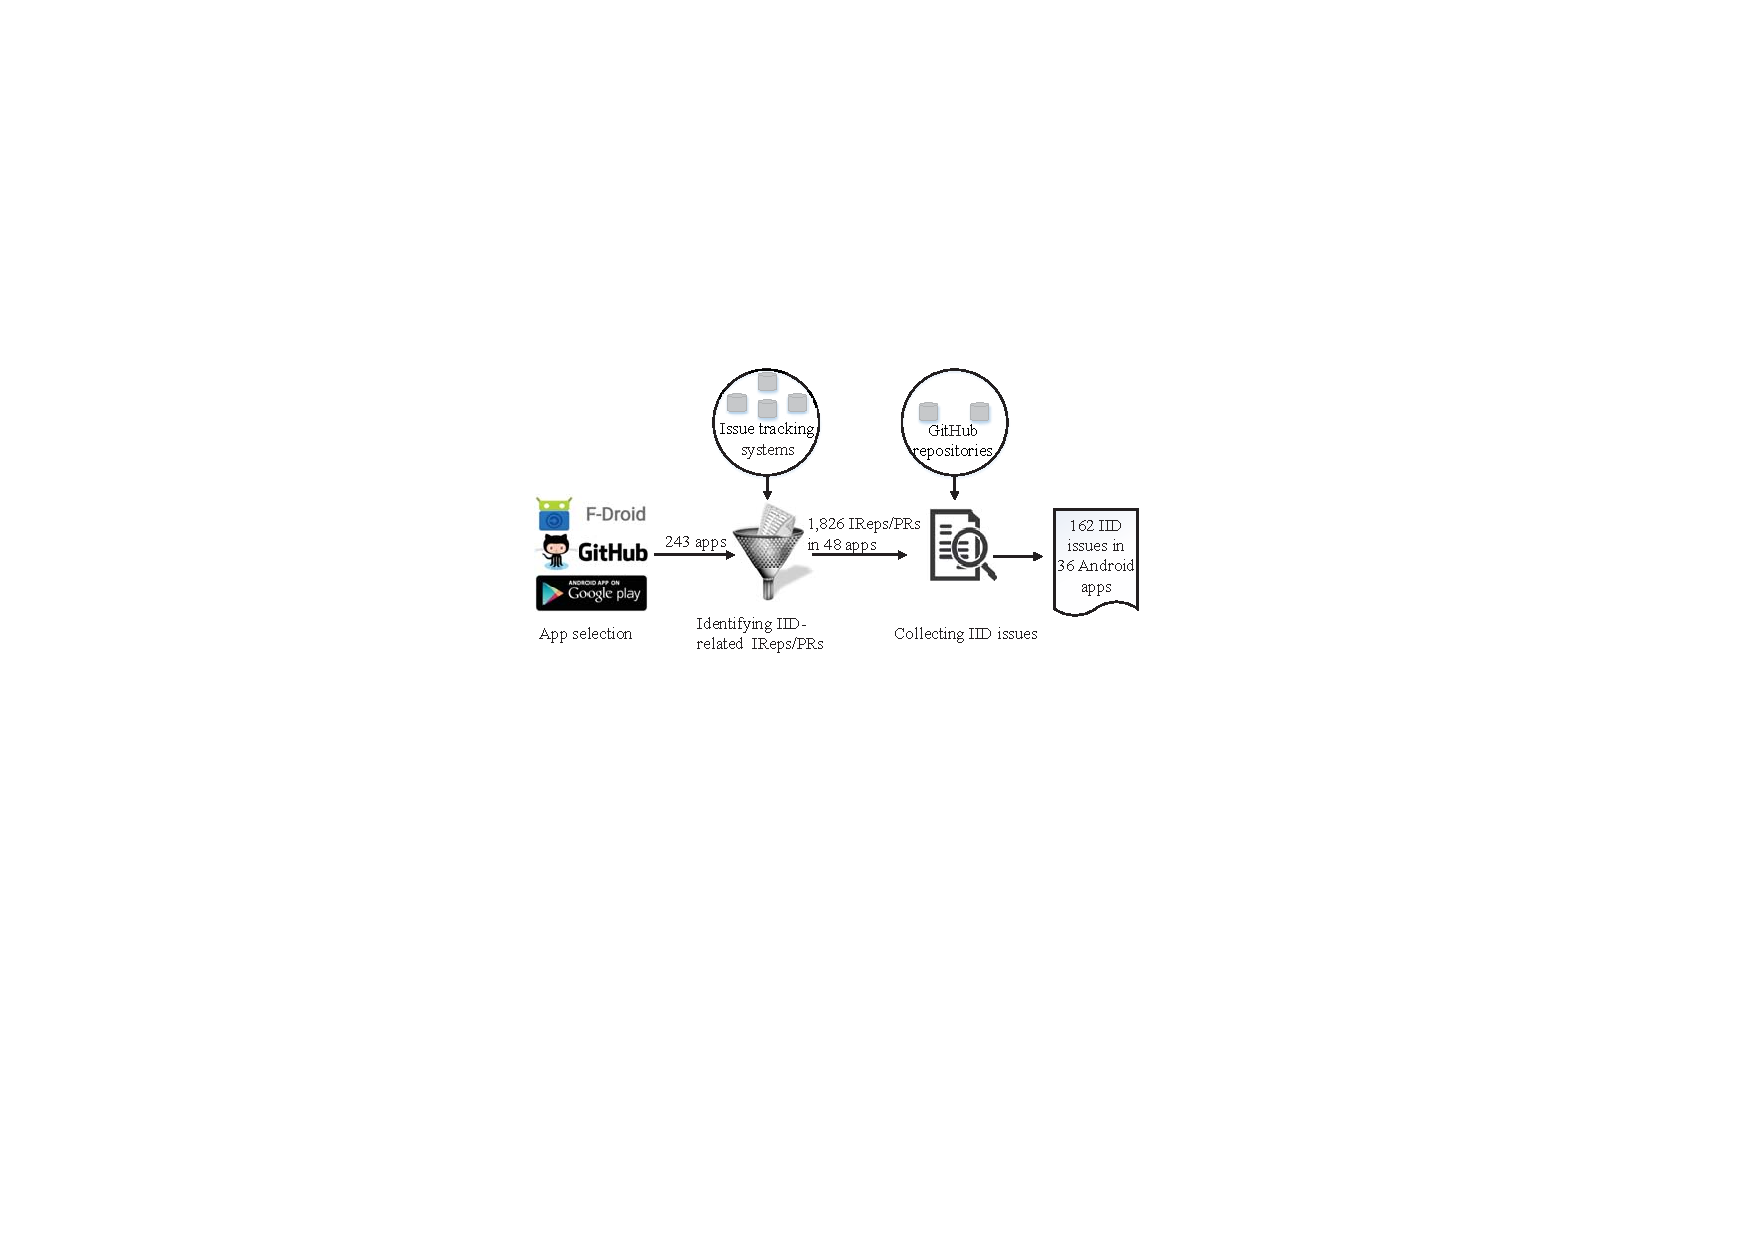
\includegraphics[scale=0.8]{pictures/fig1}
  \caption{The IID issue collection process}
  \label{fig:issue_collection}
\end{figure}

\noindent\textbf{App selection.} We selected all 243 Android apps from 1,093 randomly selected Android apps in F-Droid~\cite{f-droid} as our study subject, meeting the following selection criteria:

\begin{enumerate}
	\item \emph{Open-source}: also hosted on GitHub with an \emph{issue tracking system} for tracing potential IID issues.
	\item \emph{Well-maintained}: having over 100 code commits in the corresponding GitHub repository.
	\item \emph{Of realistic usage}: having over 1,000 downloads on the Google play market.
\end{enumerate}

\medskip

\noindent\textbf{Identifying IID-related issue reports and pull requests.}
An app user's \emph{issue report} (IRep for short) usually denotes a manifested app bug from end users.
An app developer's \emph{pull request} (PR for short), on the other hand, possibly contains the developer's perspective on a concerned app bug. Therefore, we collected both of them in the empirical study.
We first identified potential IID-related IReps and PRs in the GitHub repositories by a keyword search in their issue tracking systems using the following keywords%
\footnote{These keywords are general natural language words related to image displaying. They come from existing research work, e.g.,~\cite{linares2015developers, wang2016profiling} and our empirical study experience.}:

\begin{Verbatim}[fontsize=\small]
image   bitmap     decode   display
picture photograph show   thumbnail
\end{Verbatim}

Any IRep or PR that contains one of the above keywords in its title, body, or comment was then manually inspected to further confirm whether it indeed \emph{fixed any performance bug}:

\begin{enumerate}
  \item The IRep's/PR's text complains about the performance degradation or more serious consequences (e.g., app crash) when performing image displaying.
  \item There is evidence that an image-related bug is fixed (e.g., the concern issue report is associated with a fixing commit ID or an accepted fixing patch), and the same issue has never been re-reported in the following three months%
  \footnote{For those issues that do not contain any explicit link to any patch, we conducted a bisect on their GitHub repositories to find potential fixing patches by following the methodology of existing work~\cite{traceability}.}.
\end{enumerate}

After the manual inspection, we obtained a total of 1,826 IReps/PRs in 48 apps, which are from 22,023 IReps/PRs returned by the keyword search from the initially selected 243 Android apps.

\medskip

\noindent\textbf{Collecting IID issues and their patches.} 
We then inspected the GitHub commits associated with the 1,826 IReps/PRs to decide whether they correspond to IID issues.
For each code patch (may patch several places or files in the concerned repository, and a commit may also contain several patches) for fixing a particular image-displaying-related performance bug that is clearly documented in the corresponding IReps/PR, we consider this patch related to a new IID issue.
As such, for each decided IID issue, we obtained a patch for fixing it and its textual descriptions in the corresponding IRep/PR, which would suffice for our further manual inspection in order to answer research questions in this study.

Finally, we collected a total of 162 IID issues (distributed in 71 IReps/PRs) in 36/243 (14.8$\%$) studied Android apps. These numbers (162 issues and 14.8\% coverage) suggest that IID issues are definitely not rare, and can be considered as common in practice and deserving an in-depth study.

\medskip

\noindent\textbf{Extracting IID issues’ code slices.(\TODO{Need to be rewritten})} 
We extracted all 162 IID issues' code slices to get a deeper understanding of them from the perspective of the whole execution process of image displaying. An IID issue's code slice is a subset of statements that directly or indirectly influence the execution of inefficient image displaying through chains of dynamic data and control dependencies, which can help users focus their attention on a subset of program statements which are responsible for the issue. The process of extracting IID issues' code slices consist of following steps:

\begin{enumerate}
	\item Obtaining the IID issue’s buggy code.
	\item Obtaining the IID issue’s issue-triggering context information based on its issue description in its related issue report and comments.
	\item Reasoning about the test input that can reveal the IID issue based on its buggy code and triggering context information.
	\item Based on the test input, reasoning about the IID issue’s (hypothetical) execution trace by examining call sequences and arguments of image displaying APIs.
	\item Extracting its code slices from the obtained execution trace. It starts with a lifecycle handler (e.g., onCreate()) or an event handler (e.g., onClick()), and ends with a statement that displays or saves (e.g., upload to a server) the image data related to the IID issue.
\end{enumerate}

\medskip

\noindent\textbf{Graphical representations of IID issues’ code slices.(\TODO{Need to be rewritten})} 

Graph-based approaches provide a good way to visualize the overall flow of control, where nodes are associated with activities and edges with control or data flow between activities. 

To provide a good way to visualize the overall flow of IID issues' execution, we un-parsed the code slice into an execution skeleton. The skeleton is a \emph{directed acyclic graph} (DAG) consisting of function nodes and directed edges. A function node represents the implementation of a functional part of image displaying (e.g., image decoding). A directed edge represents an execution order. The functional parts of image displaying include:
\begin{enumerate}
	\item \emph{Image decoding}: Decoding an image into an Android-recognizable in-memory object (e.g., Bitmap, Drawable, and BitmapDrawable) and represented by green blocks.
	
	\item \emph{Image resizing}: Decoding an image into an Android-recognizable in-memory object (e.g., Bitmap, Drawable, and BitmapDrawable) and represented by yellow blocks.
	
	\item \emph{Image disk caching}: Adding an image to a disk cache and represented by orange blocks.
	
	\item \emph{Image memory caching}: Adding an image to a disk cache and represented by orange blocks.
	
	\item \emph{Image rendering}: Displaying an image object on an Android device’s screen    and Represented by blue blocks  
\end{enumerate}

\subsubsection{Analyzing the IID issues} \label{subsec:issue-analysis}

The analysis of collected IID issues is organized around the following research questions:

\smalltitle{RQ1} \emph{What are the triggering conditions and consequences of IID issues?}

RQ1 concerns user-perceived manifestation condition and consequences of IID issues, 
and thus is answered by inspecting the textual information in the titles, bodies, and comments of the collected IReps and PRs.
Recall that since all collected issues contain clear consequence descriptions,
we only need to archive them and extract their triggering conditions through these descriptions. We can further confirm the correctness of the description by analyzing their patches.

\smalltitle{RQ2} \emph{What are the root causes of IID issues?}

The root causes are extracted by a hypothetical execution of these apps. For most IID issues containing known IID-inducing triggering conditions (displaying lots of images or large images), we take these known conditions as their input. For the other IID issues, we infer their triggering conditions (one image or lots images) by analyzing their patches.
We reason about the (hypothetical) execution traces by examining call sequences and arguments of image displaying APIs,
and extract characteristics of these traces as root causes of the IID issues.

\smalltitle{RQ3} \emph{Are there common anti-patterns for IID issues?}

We inspect the patches of investigated to find whether there are common anti-patterns correlated to IID issues.
We are particularly interested in \emph{code} patterns which can facilitate lightweight static \code{lint}-like checkers.

\smalltitle{RQ4} \emph{How did developers inappropriately implement image displaying?}

Understanding different inappropriate implementation types and investigating the frequency of each considering inappropriate implementation type of IID issues can assist IID issue detection approaches or developers in locating IID issues in mobile apps. We investigated how developers implement inefficient image displaying at code level based on IID issues' code slices and patches.

\smalltitle{RQ5} \emph{How did developers fix IID issues?}

Historical IID issue fixing data can be used by automatic tools to perform IID issue fixing and also provide useful fixing suggestions to developers. Thus, we decided to perform a manual investigation on the fixing actions of IID issues, such that we gain a deeper understanding of IID issues and find repeated patterns that can be used by other automatic fixing tools or developers.

%\smalltitle{RQ6} \emph{What are the distribution of IID issues in the process of image displaying?(\TODO{Need to be rewritten})}

%An important step towards understanding IID issues is to find out where they are located. In this research question, we study the distribution of IID issues in the process of image displaying. Knowing these might help developers prioritize their efforts when identifying and fixing IID issues.

%To answer this research question, we first divided the image displaying process into multiple functional blocks. Then, we analyzed the functional block distribution of each IID issue.

